\chapter{Introduction}
The dissertation presents a simulation framework for Intelligent Transportation System (ITS). The novelty of the work is the framework distributes the computation of the actor's (vehicle and roadside infrastructure)mobility and behaviour models (i.e., the actors involved in the simulation are distributed over the network) and establishes communication via a socket. Carla \cite{carla}, an autonomous driving simulator, serves as a centralized simulation environment, and the actors are spawned in the simulation as clients using the Application Programming Interface (API) provided by the framework. Carla simulates the vehicle's movement based on the vehicle control provided by its mobility model. The distributed environment created by the framework looks similar to figure \ref{fig:my_label}.

\begin{figure}[h!]
    \centering
    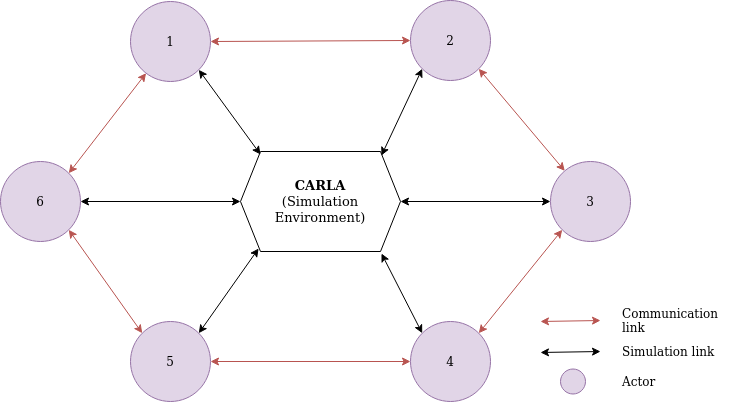
\includegraphics[width=8cm]{Framework/Images/Arc1.png}.
    \caption{Simulation Environment}
    \label{fig:my_label}
\end{figure}

\section{Motivation}
Transportation is essential for our economy and society. A country's economic, social, and political life depends upon an effective transport system. Transport is a cornerstone of European integration and crucial for the free flow of citizens, services, and goods to be served. It is also a significant contributor to the economy, accounting for about 664 billion Euros in Gross Value Added in 2017 (i.e. 5\% of the total EU's GVA) and employed over 11 million people \cite{001}. 

According to the “Statistical pocketbook 2019” of European Commission \cite{001}, 50.1\% of total freight transportation were made via roadways. Nearly 73\% of passengers made their journey through road and among them, almost 90\% of them made the road trip by car. These statistics help us to understand the importance of roadways. The increase in traffic volume creates demand and eventually leads to traffic congestion across the EU. Due to traffic congestion, a driver spends approximately 28 hours in traffic every year. Additionally, it also creates environmental and economical impacts.

Traffic congestion usually occurs when traffic flow exceeds the road capacity. Many factors can cause traffic congestion, but infrastructure stands at the top.  A simple traditional solution to reduce congestion is expanding the infrastructure. However, this is not an effective or economically reasonable solution because one cannot keep on extending as demand increases. Preferably, utilizing the infrastructure capacity to the fullest is more efficient and rational. 

ITS helps us to address congestion by continuously monitoring and regulating the traffic flow. For instance, consider a junction with traffic signals that have fixed time to switch signal. They are only effective for the ideal traffic flow, when the traffic flow decreases
the driver has to wait till green and the traffic signal creates congestion as the traffic flow increases. On the other hand, ITS can help the traffic signals dynamically adjust the switching time depending on the traffic flow.

ITS components are installed in the vehicles and along the roadside to collect traffic data, guide and control the flow. Real-world traffic scenarios are complex, highly dynamic. Because of these reasons, it must be tested and evaluated before real-world deployment. Else, they may lead to a serious problem instead of avoiding congestion. 

Including a simulator in the development cycle of ITS will help us to evaluate the system in all possible scenarios by testing it in the simulation environment mirroring real-world ITS.  Using simulators to test and evaluate ITS is cost-effective and risk-free compared to build a real-world test site.

\section{Project Overview}
\subsection{Intelligent Transportation System}
A set of different applications that use state-of-the-art technologies to monitor and regulate the traffic flow are known as ITS. Throughout the world, many countries have designed and developed ITS, and they have unique visions and goals to improve infrastructure applying ITS. Despite counties having different perspective toward ITS, they share the common goal to improve the current transportation infrastructure. This dissertation follows the standards and architecture of ITS proposed by the European Union \cite{etsi}.

\subsection{Approach}
To simulate the ITS, we need a road network, traffic infrastructure, mobility model to control vehicle behaviour, traffic demand to generate traffic flow and network model to create a communication infrastructure. 

Traffic simulators like SUMO \cite{SUMO2018}, PVT-Vissim \cite{vissim}, etc.  can create road infrastructure and simulate traffic flow based on demand and vehicle behaviour, but they do not support communication between vehicles. On the other hand, network simulators like ns3 \cite{ns3}, OMNET++ \cite{omnet}, etc. can create network infrastructure and simulated realistic communication, but they do not support mobility. Therefore, traffic simulators and network simulator should be coupled through a TCP link to create an ITS simulation environment. 

The above-mentioned simulators have to be extended for developing a customised TMS like Cooperative Adaptive Cruise Control (CACC) \cite{cacc}, platooning, slot-based driving \cite{slot-based}, etc.  For example, PLEXE \cite{plexe} implemented a platooning application by extending the Viens\cite{veins} framework (Viens is a vehicular network simulation framework created by coupling SUMO and OMNET++). The framework to simulate the ITS environment for developing TMS will be similar to the figure. 

This framework performs space-continuous and time-discrete simulation ( i.e. it updates the simulation after every time step). 
After each time step, the traffic simulator computes the behaviour of all vehicles based on the network simulation results to update the vehicle states and generate movement trace. Then, it sends the movement trace to network simulator. The network simulator updates the position of all nodes based on the received movement trace, simulates the communication and sends the result back to the traffic simulator. The sequence diagram in the figure illustrates this process. The approach lacks implementing the distributive nature of ITS and can only perform time-discrete simulation, but in real scenario time is continuous.

This dissertation introduces a framework that uses only Carla, autonomous driving simulator for simulating ITS. The framework is created by extending the Client API of Carla. Based on the traffic demand, vehicles are added as Carla client using the framework. The distributed network formed by the clients creates the communication infrastructure. 

In the proposed approach, peer to peer socket communication is used to exchange messages instead of simulating it. Each client node is responsible for its behaviour computation based on the messages it receives. This framework is capable of performing a time-continuous simulation with the help of Carla Server's asynchronous mode. Thus, it can be used to create a more realistic ITS simulation.


\subsection{Research Aims}
The research intends to design and develop a simulation framework for ITS, that creates a realistic and distributed simulation environment. The main motive is to help developers to concentrate on developing and evaluating traffic management system (TMS) models. Apart from the above, the specific objectives of this dissertation is to evaluate the feasibility of the proposed approach by creating customised scenarios using the designed framework

\subsection{Project Scope}
The dissertation focuses on designing a approach to developing a simulation framework using only an autonomous driving simulator
to create an environment closely resembling real-world ITS. Especially focuses on simulating and evaluating an actor's behaviour while developing new traffic management systems in a distributed environment. 

The framework distributes computation of the actor's behaviour among several nodes in a network and exchanges information between them through socket communication. This dissertation is not concerned about implementing the network infrastructure or underlying protocols involved in vehicular communication. 
\subsection{Benefits of this Research}
The benefit of this research is to improve the testing and evaluation processes involved while developing TMS and ITS. 
\subsection{Road Map}
The rest of this dissertation is divided into four parts, starting with chapter 2 that provides the necessary background information for this work and the state-of-the-art simulation framework for testing ITS. Chapter 3 is about the design of the framework and decisions that lead to the development of the proposed approach. The following chapter explains the architecture of the framework and APIs provided for creating custom scenarios using the framework. Chapter 5 will discuss the evaluation of the framework. Finally, the dissertation concludes with an outline stating the pros and cons of this work and future work to enhance the framework.
